%!TEX root = ../authorinstr.tex

\section{Introduction}

Designing an optimal controller for a given environment and goal can be a complex task. Reinforcement Learning (RL) techniques exist to address these tasks by learning a policy that results in choosing optimal actions in a given state. This way agents are able to learn complex behaviour, such as playing backgammon \cite{tesauro2002programming} or chess \cite{baxter1999knightcap},
real life quadripedal walking \cite{kohl2004policy}, or playing the ancient game Go \cite{alphago}.   

In initial stages the agent performs random actions while learning to approximate received reward after the chosen actions. This should enable the agent to learn an optimal policy for the defined reward function. For this learning process multiple techniques exist. The performance of a recently published technique, Neural Fitted Actor Critic (NFAC), will be compared to two well-established RL techniques: State Action Reward State Action (SARSA) and Continuous Actor Critic Learning Automaton (CACLA). All these techniques will be using a Multilayer Perceptron (MLP) as a function approximator. Previous research \cite{zimmer2016neural} indicates that for two different continuous state space environments NFAC learns a better quality policy than CACLA, which is state-of-the-art at the time of writing. Previous research \cite{nichols2015continuous} has also shown that that SARSA for continuous state spaces has achieved comparable performance to CACLA. Therefore we expect NFAC to outperform both CACLA and SARSA in terms of policy quality in continuous environments.

Recently new environments have arisen for agents to engage in, such as OpenAI \cite{openaigym}. Here multiple environments are presented, including Atari games and more classical environments such as MountainCar and CartPole. In this work, the continuous variants of the LunarLander and MountainCar environments are used. Depictions of the environments are shown in figure \ref{fig:mountainlunar}. Here both the action space and state space are continuous.  Discrete state spaces are known to work well with RL techniques, although continuous state spaces with the usage of an MLP often present more of a challenge \cite{cetina2008multilayer}. \\
%\subsection*{SARSA}
In \cite{nichols2015continuous}, Nichols et al. an approach of using SARSA together with a technique based on Newtons Method (NM) to obtain continuous action selection is used. In this work SARSA will be used in a similar way. Instead of using NM for continuous action selection, Gradient Descent (GD) is used to obtain actions resulting in a higher expected Q-value.

%\subsection*{CALCA & NFAC}
In \cite{van2007reinforcement}, two exploration techniques are discussed in CACLA: Epsilon Greedy and Gaussian Exploration. This work uses Gaussian Exploration in order to get an action close to the current optimal action. NFAC \cite{zimmer2016neural} is a method derived from CACLA. It uses the same action selection procedure as CACLA, but uses offline updates rather than the online updates CACLA uses. 



%Furthermore the required level
%of discritization can not be known in all 11 cases, and having to discover it is time intensive \cite{van2007reinforcement}. %citatie naar de cacla paper
%This potential problem can be solved by keeping the state and action space continuous in the environment representation of the agent. \\
%Several new reinforcement learning algorithms and adaptations of existing reinforcement algorithms were developed to model continuous
%state and action spaces. In this paper we will benchamark one such algorithm, named Neural Fitted Actor Critic (NFAC), which was develeped in August 2016 \cite{zimmer2016neural}
%against two established (at the time of the writing of this paper) continuous reinforcement learning algorithms, named CACLA (Continuous Actor Critic Learning Automaton)
%\cite{van2007reinforcement}
%and SARSA (State Action Reward State Action) adapted for continuous state- and action-spaces \cite{nichols2014application} with gradient descent (referred to in this paper as GD-SARSA). \\
First a formal background will be given on Connectionist Reinforcement Learning with the use of Multi-Layer Perceptrons (MLP) as function approximators, and on extending this to deal with continuous state and action spaces. In later sections the implementation of the three algorithms that are compared in this paper are explained in detail. After that, setup of the experiments will be discussed. Finally the results will be presented and evaluated, and the final conclusions will be drawn regarding the performance of NFAC compared to CACLA and GD-SARSA.

\begin{figure}[t]
 \centering 
    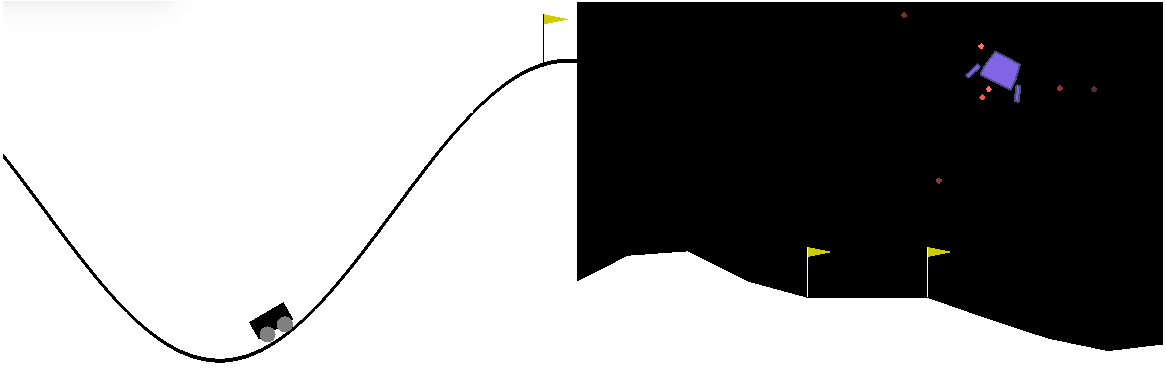
\includegraphics[width = 0.7\columnwidth]{figs/mountainlunar.png}
 \caption{Left: MountainCar Environment, Right: LunarLander Environment.}
\label{fig:mountainlunar}
\end{figure}
